\documentclass[10pt,graphicx,caption,rotating]{article}
\textheight=24cm
\textwidth=18cm
\topmargin=-2cm
\oddsidemargin=0cm
\usepackage[utf8x]{inputenc}
\usepackage[activeacute,spanish]{babel}
\usepackage{amssymb,amsfonts}
\usepackage[tbtags]{amsmath}
\usepackage{pict2e}
\usepackage{float}
\usepackage[all]{xy}
\usepackage{graphics,graphicx,color,colortbl}
\usepackage{times}
\usepackage{subfigure}
\usepackage{wrapfig}
\usepackage{multicol}
\usepackage{colortbl}
\usepackage{cite}
\usepackage{url}
\usepackage[tbtags]{amsmath}
\usepackage{amsmath,amssymb,amsfonts,amsbsy}
\usepackage{bm}
\usepackage[centerlast, small]{caption}
\usepackage[colorlinks=true, citecolor=blue, linkcolor=blue, urlcolor=blue, breaklinks=true]{hyperref}

\begin{document}
\title{Enlace de Radio Frecuencia}
\author{David Ricardo Martínez Hernández Código: $261931$\\
	Jairo Andrés Neuta Bernal Código: $261227$\\
	Oscar Andres Urbano Vallejo Código: $261683$}
\date{}
\maketitle

\begin{abstract}
\noindent
En este documento se presenta la propuesta de metodología de diseño ,  haciendo énfasis en las etapas que se requiere para la comunicación digital ASK inalámbrica de una señal analógica, en el que se hará uso de diversas tapas en la que se sensará una señal analógica, se le hará su correspondiente acondicionamiento de señal para poder así ser manipulada digitalmente,  modulada y transmitida inalámbricamente a otro punto en donde luego de su recepción, su demodulación se acondicionara nuevamente la señal para ser leída e interpretada mediante un instrumento analógico. 
\end{abstract}

\section{Planteamiento del problema}
\noindent
Las comunicaciones inalámbricas han sido utilizas mucho en los últimos años para poder controlar o sensar algunas situaciones específicas, como lo es el control de temperatura de un lugar, también las comunicaciones de radio frecuencia como las estaciones de radio, de televisión análoga y hasta de comunicaciones celulares.\\
Para ello se quiere realizar la recepción de sonido y poderlo transmitir por medio del la modulación digital \textbf{ASK} a un parlante. Para lograr esta modulación es necesario hacer uso de las herramientas adquiridas a lo largo de la carrera y así poder realizar dicha modulación con el mayor éxito posible.

\section{Objetivos}
\subsection{Objetivo General}
\begin{itemize}
 \item Realizar una comunicación ASK de una señal análoga y replicarla en un parlante.
\end{itemize}
\subsection{Objetivos Específicos}
\begin{itemize}
 \item Realizar la discretización de la señal análoga por medio de un conversor análogo digital (\textbf{ADC}).
 \item Realizar la conversión paralelo a serial de la señal análoga discretizada y la conversión serial paralelo de la misma señal.
 \item Realizar la modulación y demodulación de la señal que es transmitida por la antena.
 \item Realizar un acople de impedancias de todo el diseño a $50\Omega$.
 \item Realizar la construcción de la señal discreitzada a la señal original por medio de un conversor digital a análogo (\textbf{DAC}).
 \item Realizar un clock a $1KHz$ para sincronizar todos los dispositivos asíncronos.
\end{itemize}

\section{Diseño}
\noindent
El diseño se ha divido en dos etapas:
\begin{enumerate}
 \item Etapa de adquisición de datos, codificación y transmisión.
 \item Etapa de recepción, decodificación de datos y visua-lización.
\end{enumerate}
\noindent
La primera de estas etapas consta de cinco submodulos;  en esta subdivisón se encuentra la recepción de la señal analógica, posteriormente una etapa de amplificación y transducción de señal mediante un modulo \textbf{ADC} que muestrea, retiene, cuantifica y codifica la señal de interés, luego se tiene la etapa de de conversión  paralelo a serie de $8$ \textit{bits}, posterior a esto se encuentra la etapa de modulación por \textbf{ASK} para la transmisión y finalmente un modulo de acople mediante una línea de transmisión coplanar, con la antena transmisora (ver figura \ref{fig1}).\\
Con respecto a la segunda etapa principal, esta también cuenta con submodulos que la componen, de tal manera el proceso inverso al que se plantea desarrollar en la primera etapa, conforme a esto se tiene, una antena receptora acoplada a una línea coplanar, que a su vez  se comunica con el demodulador  seleccionado para esta aplicación,  posterior a esto la señal  demodulada pasa por el modulo de conversión de $8 bit$ paralelo a serie, luego se realiza  un proceso de  conversión digital análogo  de la señal,000000000000000 por medio de un \textbf{DAC} y finalmente para efectos de manipulación y lectura de la señal analógica, se pasara la señal por un modulo de amplificación y percepción con un parlante (ver figura \ref{fig4}).

\subsection{Primera Etapa}

\begin{figure}[H]
	\centering
		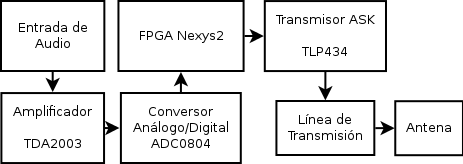
\includegraphics[scale=0.55]{Diagrama1.png}
	\caption{Etapa de adquisición de datos, codificación y transmisión.}
	\label{fig1}
\end{figure}

\subsubsection{Adquisición de datos}
\noindent
Como se observa en la Figura \ref{fig1} la primera etapa empieza con la obtención del sonido, esta se hará por medio un celular, según la caracterización realizada la salida del celular el cual se encuentra entre  $0 V$ y $50 mV$.\\ 
Sin embargo el conversor \textbf{ADC} funciona para señales de entrada comprendidas entre $0V$ y $5V$ por tal motivo se realiza una etapa de amplificación de la señal de entrada.

\subsubsection{Amplificador de Voltaje}\label{amp}
\noindent
El amplificador de voltaje es un amplificador $TDA2003$ el cual es usado comúnmente como amplificador de audio, apoyado en su entrada por un filtro pasabajas. Este amplificador permite que la señal de entrada al \textbf{ADC} se encuentre entre $0 V$ y $5 V$, esto se realizó con el fin de poseer una mejor resolución a la hora de convertir la señal análoga a digital. 

\subsubsection{Conversor Análogo Digital} \label{ADC}
\noindent
El $ADC 0804$ (Figura \ref{fig2}) puede ser alimentado con $5 V$, esto garantiza un muestreo óptimo para la señal de entrada que se esta utilizando, cuenta con una salida de $8$ bits lo cual da lugar a una resolución de $256$ posibles valores, por lo cual con dicha polarización será capaz de detectar cambios a la entrada  hasta de $20mV$.
\begin{figure}[H]
	\centering
		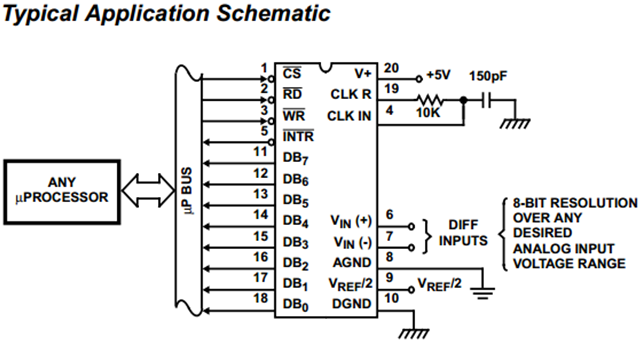
\includegraphics[scale=0.4]{ADC.png}
	\caption{Diagrama esquemático del $ADC0804$.}
	\label{fig2}
\end{figure}
\noindent
La tasa de conversión puede ser variada en función de los elementos conectados entre los pines  4 y 19 sin embargo para el montaje típico mostrado en la figura Figura \ref{fig2} se cuenta con una Tasa de conversión de $f_{CLK} = 640kHz$.

\subsubsection{Conversor Paralelo Serial}
\noindent
Esta etapa se va a realizar por medio de la \textbf{FPGA} por medio de un software implementado en ella
%Por medio del conversor $74HC175$ la señal obtenida del $ADC0804$ de $8$ bits es convertida a una señal serial de $1$ solo bit que contiene toda la información de los $8$ bits del \textit{ADC}. Este circuito es prácticamente un registro de desplazamiento,  funcionara con una señal de clock  de $1 KHz$ de frecuencia lo que hará que el bit serial que se transmita tenga una frecuencia de $1Kbps$,tasa de bits con la que funciona  el par transmisor receptor.  La señal de clock será suministrada por el circuito mostrado en la Figura \ref{fig3} en el cual se utiliza el integrado $LM555$ para formar el oscilador.
%\begin{figure}[H]
%	\centering
%		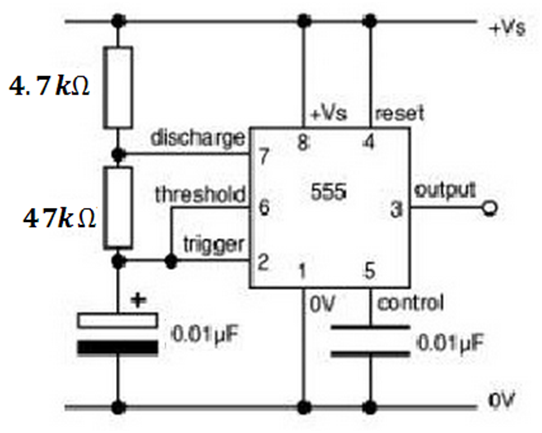
\includegraphics[scale=0.45]{555.png}%
%	\label{fig3}
%\end{figure}

\subsubsection{Transmisor ASK}
\noindent
Para este caso se utilizó un $TLP434A$. Este transmisor es alimentado con $5 V$, opera con una tasa de bits de $1 Kbps$, este circuito se encarga de hacer la modulación y genera la onda que será llevada a la antena, esta referencia en específico modula la señal con una portadora de $434 MHz$, frecuencia central a la que será transmitida la información en el aire; se escogió el par transmisor receptor en esta frecuencia de operación ya que está comprendida en la banda destinada a los radio aficionados ($430 MHz – 440 MHz$).

\subsubsection{Línea de Transmisión} \label{LTx}
\noindent
Como es necesario utilizar una línea de transmisión para realizar las conexiones correspondientes se utilizo un arreglo de líneas para poder acoplar la unión del modulador con la antena, este acople debe estar diseñado a $50\Omega$ porque todos los elementos del circuito también lo están.\\
Se utilizaron dos líneas de microcinta acopladas, tienen una longitud de $l_1=50 mm$, un ancho de $w_1=1.33877mm$ y una distancia $s_1=1.2 mm$, asumiendo un $\epsilon _R = 4.34$, espesor del dieléctrico de $H=0.711mm$, y un ancho de la pista de cobre de $T=35 \mu m$.\\
Estos resultados se obtuvieron con el simulador \textbf{Qucs $0.0.16$}.

\subsubsection{Antena}
\noindent
Suministrada por el docente, se sabe que tiene una impedancia de $50 \Omega$.

\subsection{Segunda Etapa}
\begin{figure}[H]
	\centering
		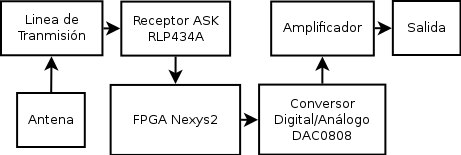
\includegraphics[scale=0.55]{Diagrama2.png}
	\caption{Etapa de recepción, decodificación de datos y visualización.}
	\label{fig4}
\end{figure}

\subsubsection{Antena}
\noindent
Suministrada por el docente, se sabe que tiene una impedancia de $50 \Omega$.

\subsubsection{Línea de Transmisión}
\noindent
Se utilizó la misma línea descrita en la etapa anterior (ver  ~\ref{LTx}).

\subsubsection{Demodulador ASK}
\noindent
Se utilizó el receptor $RLP434$ que es el receptor compatible con el transmisor $TLP434A$. Trabaja a la misma frecuencia de operación ($434 MHz$) y con la misma tasa de bits ($1Kbps$), el receptor además demodula la señal y entrega el bit serial que contiene la información del sonido.

\subsubsection{Conversor Serial Paralelo}
\noindent
Esta etapa sera realizada por la \textbf{FPGA}
%Se utilizará el conversor Serial Paralelo $74HC164$. Que trabajara a la misma frecuencia de operación que el $ADC$ (ver  ~\ref{ADC})) utilizado en la primera etapa de diseño, por tanto utilizara el mismo circuito de la Figura \ref{fig3} para obtener la señal de clock de $1KHz$.

\subsubsection{Conversor Digital Análogo}
\noindent
Se utilizará el conversor Digital-Análogo $DAC0808$.

\subsubsection{Amplificador de Voltaje y Salida}
\noindent
Se utilizó un juego de parlantes alimentados por un cargador de celular, los cuales ya tienen integrado un amplificador de voltaje integrado.

\section{Costos}
\noindent
Para realizar este proyecto se van a utilizar estos recursos:
\begin{table}[H]
	\centering
\begin{tabular}{|c|c|r|r|}\hline
 \textbf{Cantidad} & \textbf{Recurso} & \textbf{Valor Unitario} & \textbf{Total} \\ \hline
 2 & Amplificadores $TDA2003$ & $3.000$ & $6.000$ \\ \hline
 1 & $ADC0804$ & $8.700$ & $8.700$ \\ \hline
 1 & $TLP434A$ & $9.300$ & $9.300$ \\ \hline
 1 & $RLP434$ & $10.100$ & $10.100$ \\ \hline
 1 & $DAC0808$ & $4.350$ & $4.350$ \\ \hline
 1 & Circuito Impreso $FR4$ & $0$ & $0$ \\ \hline
 1 & Circuito Impreso $10 cm * 10 cm$ & $3.500$ & $3.500$ \\ \hline
 2 & Metro de Ribbun & $2.000$ & $4.000$ \\ \hline
 8 & Conectores para Ribbun & $1.500$ & $12.000$ \\ \hline
 10 & Condensadores & $500$ & $5.000$ \\ \hline
 10 & Resistencias & $100$ & $1.000$ \\ \hline
 2 & Conectores & $2.000$ & $4.000$ \\ \hline
 1 & Plugin de audio & $3.000$ & $3.000$ \\ \hline
 1 & Diodo $1n4004$ & $200$ & $200$ \\ \hline
 1 & Diodo Zener & $400$ & $400$ \\ \hline
 2 & FPGA Nexys2 & $400.000$ & $800.000$ \\ \hline
    \end{tabular}
	\caption{Costos de implementación.}
	\label{tab1}
\end{table}
\noindent
Para realizar este proyecto es necesario hacer una inversión de aproximadamente $\$ 871.500$, sin tomar en cuenta las horas de diseño por cada integrante del grupo.

\section{Conclusiones}
\begin{itemize}
 \item .
 \item .
 \item .
\end{itemize}

\bibliographystyle{ieeetran}
\begin{thebibliography}{99}

\bibitem{balanice} Balanice, Constantine A.
{\em ``Antenna theory analysis and desing''}.
John Wiley \& Sons, Inc., Third Edition, 2005

\bibitem{pozar} Pozar, David M.
{\em ``Microwave Engineering''}.
John Wiley \& Sons, Inc., Fourth Edition, 2012

\bibitem{page1} Sitio web: \url{http://www.sigmaelectronica.net}, visitado el 04 de junio de 2013.

\bibitem{page2} Sitio web: \url{http://www.tekcien.com}, visitado el 04 de junio de 2013.

\bibitem{page3} Hoja de datos del $TDA2003$: \url{http://pdf.datasheetcatalog.com/datasheet2/8/0iyjghfjy8fhfz8jkwkgedw8qsky.pdf}, leída el 04 de junio de 2013.

\bibitem{page4} Hoja de datos del $ADC0804$: \url{http://www.sigmaelectronica.net/manuals/ADC0804.pdf}, leída el 04 de junio de 2013.

\bibitem{page5} Hoja de datos de la $FPGA$ $Nexys2$: \url{http://www.digilentinc.com/Data/Products/NEXYS2/Nexys2_rm.pdf}, leída el 04 de junio de 2013.

\bibitem{page6} Hoja de datos del $TLP434A$: \url{http://www.sigmaelectronica.net/manuals/TLPRLP434A.pdf}, leída el 04 de junio de 2013.

\bibitem{page7} Hoja de datos del $RLP434$: \url{http://www.sigmaelectronica.net/manuals/tlprlp434.pdf}, leída el 04 de junio de 2013.

\bibitem{page8} Hoja de datos del $DAC0808$: \url{http://www.sigmaelectronica.net/manuals/DAC0808.pdf}, leída el 04 de junio de 2013.

\bibitem{page9} Sitio web: \url{http://www.microelectronicos.com/datasheets/MO-RX3400.pdf}, visitado el 04 de junio de 2013.

\bibitem{page10} Sitio web: \url{http://www.microelectronicos.com/datasheets/MO-SAWR.pdf}, visitado el 04 de junio de 2013.

\end{thebibliography}
\end{document}